\documentclass[tikz]{standalone}

\usepackage{tikz}
\usetikzlibrary{arrows.meta}
\usetikzlibrary{calc}
\usetikzlibrary{decorations.pathreplacing}

%\usepackage{helvet}
%\renewcommand{\familydefault}{\sfdefault}

% \usepackage[default]{comfortaa}
% \usepackage[T1]{fontenc}

\usepackage[T1]{fontenc}
\usepackage[default]{raleway}

%%%%%%%%%%%%%%%%%%%%%%%%%%%%%%%%%%%%%%%%%%%%%%%%%%%%%%%%%%%%%%%%%%%%%%%%%%%%%%%%
%% COLORS
%%%%%%%%%%%%%%%%%%%%%%%%%%%%%%%%%%%%%%%%%%%%%%%%%%%%%%%%%%%%%%%%%%%%%%%%%%%%%%%%
\definecolor{grey} {rgb}{ 0.557 , 0.557 , 0.557 }
\definecolor{line0}{rgb}{ 0.259 , 0.282 , 0.784 }
\definecolor{line1}{rgb}{ 0.329 , 0.757 , 0.341 }
\definecolor{line2}{rgb}{ 0.906 , 0.816 , 0.122 }
\definecolor{line3}{rgb}{ 0.576 , 0.282 , 0.145 }
\definecolor{line4}{rgb}{ 0.882 , 0.427 , 0.098 }
\definecolor{line5}{rgb}{ 0.765 , 0.129 , 0.129 }

\colorlet{player0}{line5}
\colorlet{player1}{line1}

%%%%%%%%%%%%%%%%%%%%%%%%%%%%%%%%%%%%%%%%%%%%%%%%%%%%%%%%%%%%%%%%%%%%%%%%%%%%%%%%
%% DIGITS
%%%%%%%%%%%%%%%%%%%%%%%%%%%%%%%%%%%%%%%%%%%%%%%%%%%%%%%%%%%%%%%%%%%%%%%%%%%%%%%%
%% -----------------------------------------------------------------------------
%% Zero
%% -----------------------------------------------------------------------------
\newcommand{\digitZero}[3]
{
  \fill[#3, even odd rule] ( #1 , #2 ) ++ ( 0 , 0 ) rectangle ++ ( 12 , 10 )
                           ( #1 , #2 ) ++ ( 4 , 2 ) rectangle ++ (  4 ,  6 );
}
%% -----------------------------------------------------------------------------
%% One
%% -----------------------------------------------------------------------------
\newcommand{\digitOne}[3]
{
  \fill[#3] ( #1 , #2 ) rectangle ++ ( 4 , 10 );
}
%% -----------------------------------------------------------------------------
%% Five
%% -----------------------------------------------------------------------------
\newcommand{\digitFive}[3]
{
  \fill[#3] ( #1 , #2 ) -- ++ (  12 , 0 ) -- ++ ( 0 ,  6 ) 
                        -- ++ ( - 8 , 0 ) -- ++ ( 0 ,  2 )
                        -- ++ (   8 , 0 ) -- ++ ( 0 ,  2 )
                        -- ++ ( -12 , 0 ) -- ++ ( 0 , -6 )
                        -- ++ (   8 , 0 ) -- ++ ( 0 , -2 )
                        -- ++ ( - 8 , 0 ) -- cycle;
}
%%%%%%%%%%%%%%%%%%%%%%%%%%%%%%%%%%%%%%%%%%%%%%%%%%%%%%%%%%%%%%%%%%%%%%%%%%%%%%%%

\begin{document}

  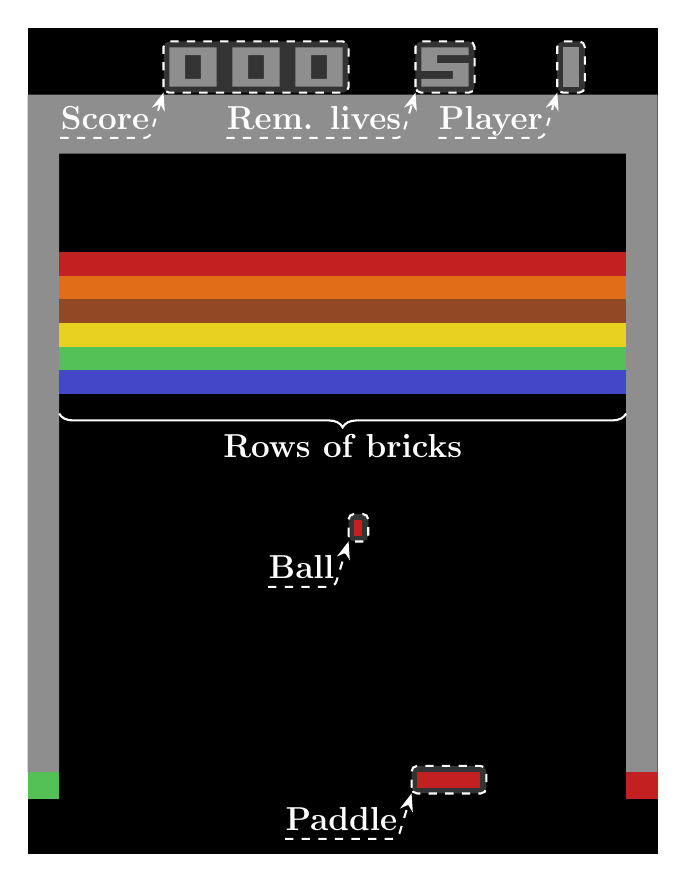
\begin{tikzpicture}[scale               = 0.05,
                      >                   = Stealth,
                      nodeStyle/.style    = { text           = white     ,
                                              inner sep      = 0pt       ,
                                              minimum height = 11pt      ,
                                              text height    = 1.5ex     ,
                                              text depth     = 0.25ex    ,
                                              font           = \large\bf },
                      pointingLine/.style = { ->, white, dashed,
                                              rounded corners = 2pt    ,
                                              line width      = 0.75pt },
                      rectStyle/.style    = { dashed                   ,
                                              draw            = white  ,
                                              fill            = white  ,
                                              fill opacity    = 0.2   ,
                                              rounded corners = 2pt    ,
                                              line width      = 0.75pt }]

    %% -------------------------------------------------------------------------
    %% Padding
    %% -------------------------------------------------------------------------
    \coordinate (PAD) at ( 1.5 , 1.5 );
    
    %% -------------------------------------------------------------------------
    %% Background
    %% -------------------------------------------------------------------------
    \fill[black] ( 0 , 0 ) rectangle ( 160 , 210 );
    
    %% -------------------------------------------------------------------------
    %% Outline
    %% -------------------------------------------------------------------------
    \fill[grey] (   0 ,  21 ) -- (   0 , 193 ) --
                ( 160 , 193 ) -- ( 160 ,  21 ) --
                ( 152 ,  21 ) -- ( 152 , 178 ) --
                (   8 , 178 ) -- (   8 ,  21 ) -- cycle;
                
    \fill[player1] (   0 , 14 ) rectangle ++ ( 8 , 7 );
    \fill[player0] ( 152 , 14 ) rectangle ++ ( 8 , 7 );
                
    %% -------------------------------------------------------------------------
    %% Score
    %% -------------------------------------------------------------------------
    \draw[rectStyle] ($(36, 195)-(PAD)$) node (score) {}
                                         rectangle ++ ($(44, 10)+2*(PAD)$);
    \digitZero{36}{195}{grey}
    \digitZero{52}{195}{grey}
    \digitZero{68}{195}{grey}
    \node[nodeStyle, anchor = north east, xshift = -5, yshift = -5]
         (scoreLabel) at (score.center) {Score};
    \draw[pointingLine] (scoreLabel.south west) -- (scoreLabel.south east)
                                                -- (score.center);
    
    %% -------------------------------------------------------------------------
    %% Life
    %% -------------------------------------------------------------------------
    \draw[rectStyle] ($(100, 195)-(PAD)$) node (lives) {}
                                          rectangle ++ ($(12, 10)+2*(PAD)$);
    \digitFive{100}{195}{grey}
    \node[nodeStyle, anchor = north east, xshift = -5, yshift = -5]
         (livesLabel) at (lives.center) {Rem. lives};
    \draw[pointingLine] (livesLabel.south west) -- (livesLabel.south east)
                                                -- (lives.center);
    
    %% -------------------------------------------------------------------------
    %% Player
    %% -------------------------------------------------------------------------
    \draw[rectStyle] ($(136, 195)-(PAD)$) node (player) {}
                                          rectangle ++ ($(4, 10)+2*(PAD)$);
    \digitOne{136}{195}{grey}
    \node[nodeStyle, anchor = north east, xshift = -5, yshift = -5]
         (playerLabel) at (player.center) {Player};
    \draw[pointingLine] (playerLabel.south west) -- (playerLabel.south east)
                                                 -- (player.center);
                                                
    %% -------------------------------------------------------------------------
    %% Bricks
    %% -------------------------------------------------------------------------
    \fill[line0] ( 8 , 117 ) ++ ( 0 ,  0 ) rectangle ++ ( 144 , 6 );
    \fill[line1] ( 8 , 117 ) ++ ( 0 ,  6 ) rectangle ++ ( 144 , 6 );
    \fill[line2] ( 8 , 117 ) ++ ( 0 , 12 ) rectangle ++ ( 144 , 6 );
    \fill[line3] ( 8 , 117 ) ++ ( 0 , 18 ) rectangle ++ ( 144 , 6 );
    \fill[line4] ( 8 , 117 ) ++ ( 0 , 24 ) rectangle ++ ( 144 , 6 );
    \fill[line5] ( 8 , 117 ) ++ ( 0 , 30 ) rectangle ++ ( 144 , 6 );
    
    \draw[white, line width = 0.75, decorate,
         decoration = { brace, amplitude = 5pt, mirror }]
         ($( 8 , 117 ) + ( 0 , -5 )$) -- ++ ( 144 , 0 )
         node[nodeStyle, midway, anchor = north, yshift = -7.5pt]
             (brace) {Rows of bricks};
 
    %% -------------------------------------------------------------------------
    %% Paddle
    %% -------------------------------------------------------------------------
    \draw[rectStyle] ($(99, 17)-(PAD)$) node (paddle) {}
                                        rectangle ++ ($(16, 4)+2*(PAD)$);
    \fill[player0] ( 99 , 17 ) rectangle ++ ( 16 , 4 );
    \node[nodeStyle, anchor = north east, xshift = -5, yshift = -5]
         (paddleLabel) at (paddle.center) {Paddle};
    \draw[pointingLine] (paddleLabel.south west) -- (paddleLabel.south east)
                                                 -- (paddle.center);
                                                 
    %% -------------------------------------------------------------------------
    %% Ball
    %% -------------------------------------------------------------------------
    \draw[rectStyle] ($(83, 81)-(PAD)$) node (ball) {}
                                        rectangle ++ ($(2, 4)+2*(PAD)$);
    \fill[player0] ( 83 , 81 ) rectangle ++ ( 2 , 4 );
    \node[nodeStyle, anchor = north east, xshift = -5, yshift = -5]
         (ballLabel) at (ball.center) {Ball};
    \draw[pointingLine] (ballLabel.south west) -- (ballLabel.south east)
                                               -- (ball.center);
                                                 
  \end{tikzpicture}
  
\end{document} 
